\chapter{Manual de usuario}
	
	Este apéndice constituye el manual de usuario del producto software desarrollado por el presente proyecto fin de carrera e incluye la información necesaria para su ejecución.
	
	\section{Instalación y desinstalación}
		
		En esta sección se realizará una explicación de cómo se podrá instalar y desinstalar la nueva funcionalidad del toolbox \textit{nnet} añadida por las nuevas funciones y la aplicación gráfica.
		
		\subsection{Instalación}
		
			Para la instalación se requerirá un descompresor, ya que todo el código fuente del toolbox se encontrará en archivo comprimido .zip como se muestra en la Figura \ref{fig:arc_com}.\\
			
			\begin{figure}[htbp]
				\centering
				
\includegraphics[scale=1]{img/arc_com.png}
				\caption{Instalación. Archivo del código fuente comprimido.}
				\label{fig:arc_com}
			\end{figure}
			
			Al descomprimir el archivo comprimido se quedará la carpeta con el código fuente, como se muestra en la Figura \ref{fig:car_src}, lista para poder añadirla al \textit{path} de Matlab.\\
			
			\begin{figure}[htbp]
				\centering
				
\includegraphics[scale=1]{img/car_src.png}
				\caption{Instalación. Carpeta del código fuente.}
				\label{fig:car_src}
			\end{figure}
			
			Para añadir el código al \textit{path} de Matlab habrá que seguir los siguientes pasos:\\
			
			Primero seleccione del menú \textit{File} y pulse sobre la opción \textit{Set Path} tal y como se muestra en la Figura \ref{fig:menu}.\\
			
			\begin{figure}[htbp]
				\centering
				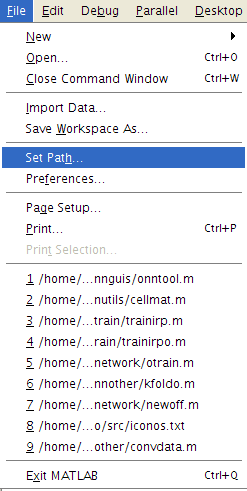
\includegraphics[scale=0.6]{img/menu.png}
				\caption{Instalación. Menú File.}
				\label{fig:menu}
			\end{figure}
			
			Aparecerá una pantalla como la que se muestra en la Figura \ref{fig:path}. En esta pantalla deberá seleccionar la opción \textit{Add with Subfolders}.\\
			
			\begin{figure}[htbp]
				\centering
				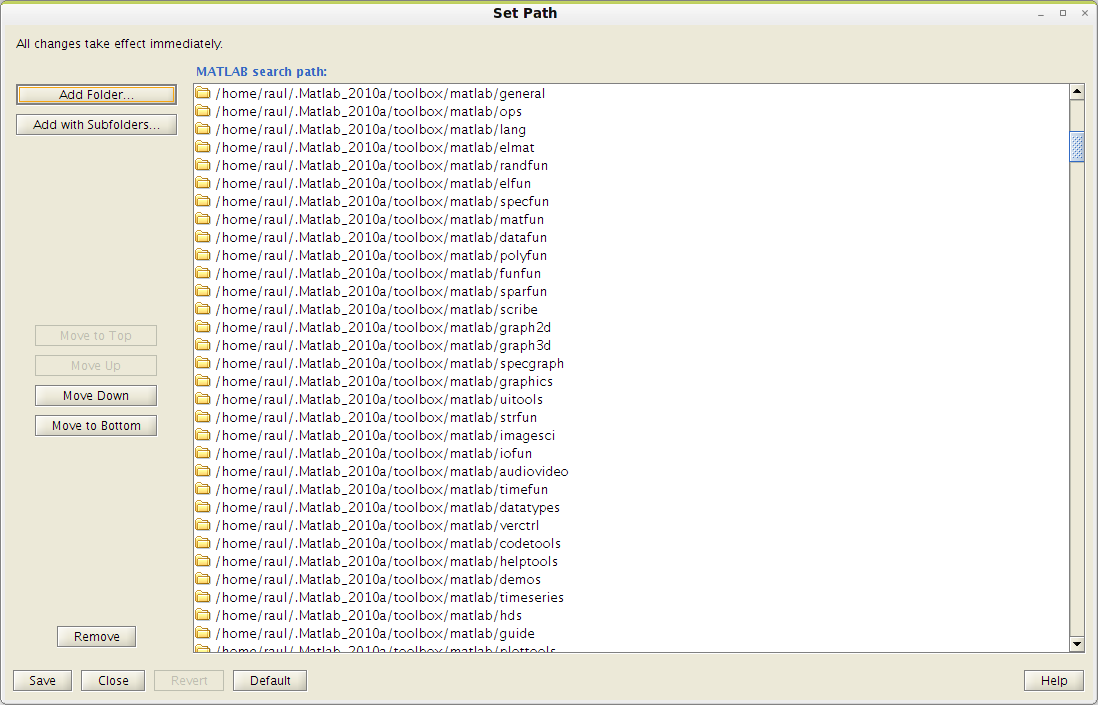
\includegraphics[scale=0.4]{img/path.png}
				\caption{Instalación. Añadir al Path.}
				\label{fig:path}
			\end{figure}
			
			En este momento aparecerá un cuadro de diálogo como el que se muestra en la Figura \ref{fig:dialog} en el que deberá seleccionar la carpeta que se ha descomprimido y que contiene todo el código fuente.\\
			
			\begin{figure}[htbp]
				\centering
				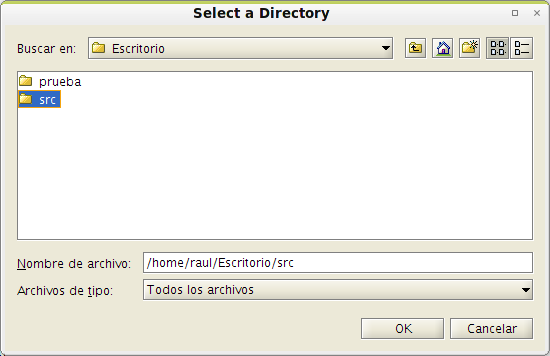
\includegraphics[scale=0.6]{img/dialog.png}
				\caption{Instalación. Cuadro de diálogo.}
				\label{fig:dialog}
			\end{figure}
			
			Al pulsar \textit{OK} del cuadro de diálogo se añadirá todo el contenido al \textit{Path} de Matlab. En este momento habrá que pulsar sobre el botón \textit{Save} y luego en \textit{Close}, con lo que ya se podrá llamar a cualquiera de las funciones del nuevo \textit{toolbox} como a cualquier otra función propia de Matlab.
		
		\subsection{Desinstalación}
		
			Para la desinstalación de la nueva funcionalidad del \textit{toolbox} para Matlab sólo habrá que realizar un paso. Como se puede observar en la Figura \ref{fig:path2}, el \textit{path} contendrá el árbol de contenidos del \textit{toolbox}, con lo que habrá que seleccionar todos los elementos y seguidamente pulsar sobre el botón \textit{Remove}. Una vez eliminado deberá pulsar sobre el botón \textit{Save} y seguidamente sobre \textit{Close} y ya estará todo desinstalado.
			
			\begin{figure}[htbp]
				\centering
				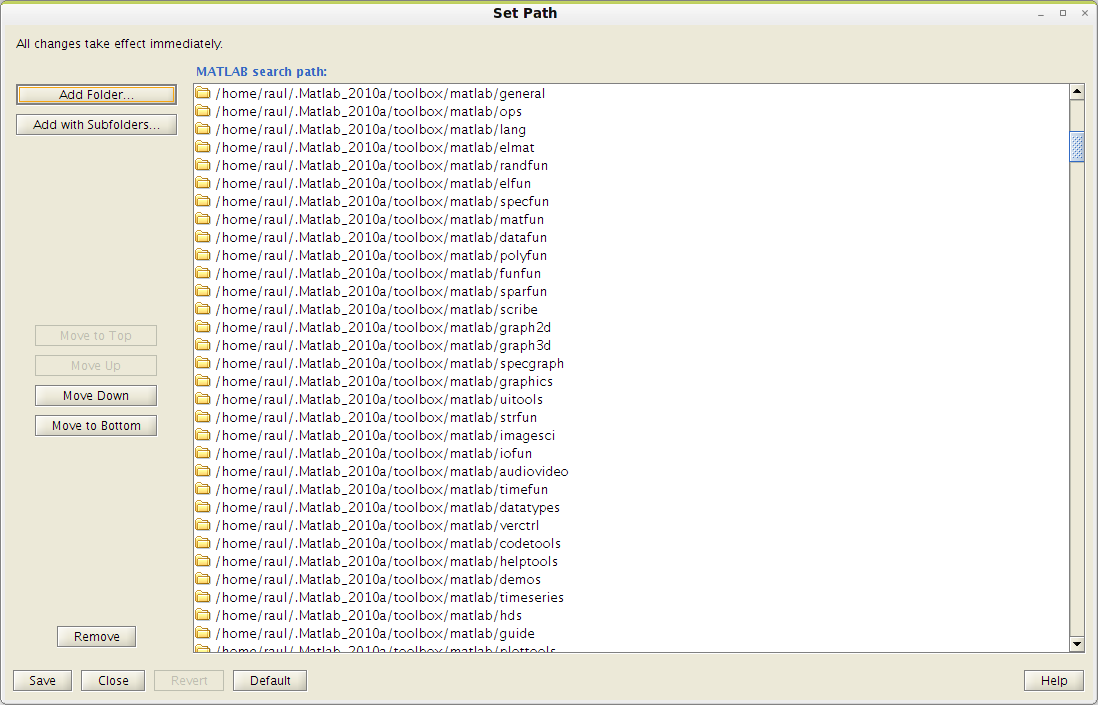
\includegraphics[scale=0.4]{img/path.png}
				\caption{Desinstalación. Eliminación de contenido del Path.}
				\label{fig:path2}
			\end{figure}
		
	\section{Uso de la aplicación}
	
		En esta sección se expondrá un ejemplo de la aplicación para que cualquiera pueda usarla. Se explicará detalladamente cada pantalla que proporciona la aplicación mostrando además una imagen de la misma.\\
		
		La primera pantalla que se verá cuando se inicia la aplicación será la pantalla inicial de bienvenida, que se muestra en la Figura \ref{fig:int01}. En esta pantalla se puede observar los siguientes elementos: una barra en la parte superior con el nombre de la aplicación ``nntool", seguidamente se muestra una cabecera en la que se ve el saludo de bienvenida a la aplicación junto a los escudos de la Universidad de Córdoba y de Ingeniería Informática. Después se muestran dos paneles, uno con información general sobre el tema que se trata y otro con información específica sobre redes neuronales ordinales. Dos de los botones que contiene esta pantalla y que contendrán el resto a partir de ahora a excepción de la última pantalla son los botones para pasar a la siguiente pantalla (Next) y para cancelar la aplicación y salirse (Cancel).\\
		
		\begin{figure}[htbp]
			\centering
			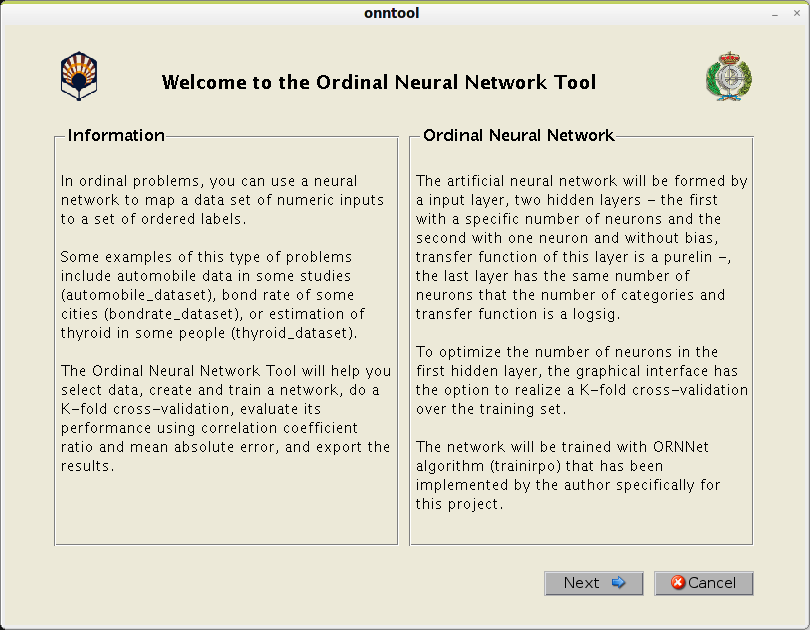
\includegraphics[scale=0.5]{interfaz/interface01.png}
			\caption{Interfaz gráfica. Pantalla de bienvenida.}
			\label{fig:int01}
		\end{figure}
		
		Al pulsar el botón siguiente (Next) se pasará a la siguiente pantalla, la pantalla de obtención de datos, la cual muestra dos paneles, uno para cargar los datos del conjunto de entrenamiento y otro para cargar los datos del conjunto de test. Estos paneles constan de un menú popup en el que se mostrarán de cada conjunto los datos de entrada (Inputs) y los datos objetivos (Targets).\\
		
		\begin{figure}[htbp]
			\centering
			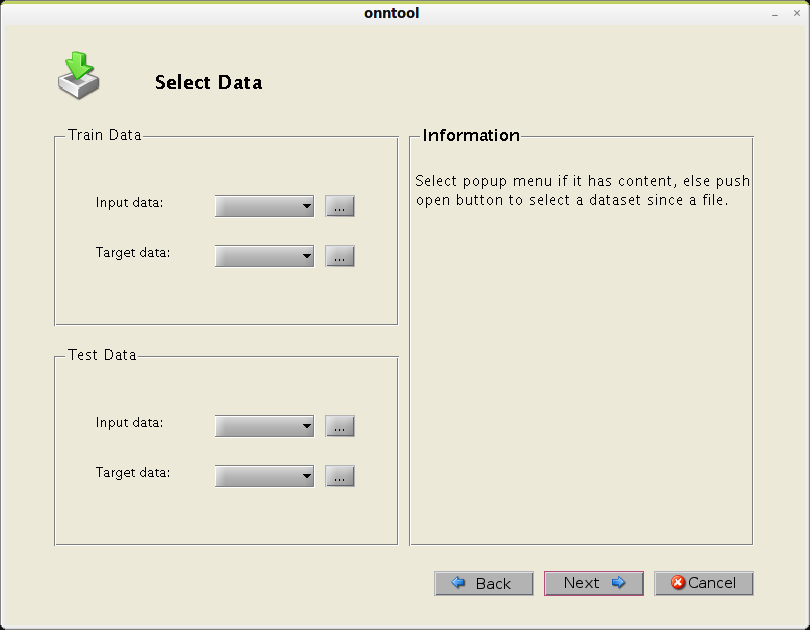
\includegraphics[scale=0.5]{interfaz/interface02.png}
			\caption{Interfaz gráfica. Pantalla de carga de datos.}
			\label{fig:int02}
		\end{figure}
		
		Si se intenta pasar a la siguiente pantalla pulsando directamente el botón siguiente (Next) sin haber cargado los conjuntos de datos, se mostrará un mensaje de advertencia como el que se muestra en la Figura \ref{fig:int02-1}.\\
		
		\begin{figure}[htbp]
			\centering
			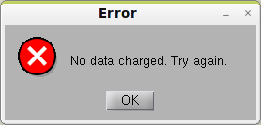
\includegraphics[scale=1]{interfaz/interface02-1.png}
			\caption{Interfaz gráfica. Aviso de falta de carga de datos.}
			\label{fig:int02-1}
		\end{figure}
		
		En caso de que no haya datos cargados previamente, habrá que pulsar alguno de los botones para abrir un cuadro de diálogo y de este modo poder cargar un conjunto de datos desde un par de ficheros (train y test). Las Figuras de la \ref{fig:int03} a la \ref{fig:int07} muestran como se puede cargar un par de ficheros de un conjunto de datos paso a paso.\\
		
		\begin{figure}[htbp]
			\centering
			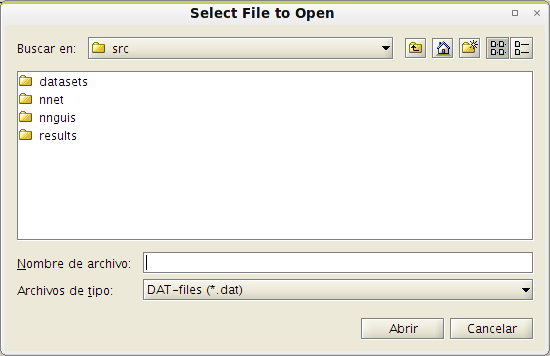
\includegraphics[scale=0.6]{interfaz/interface03.png}
			\caption{Interfaz gráfica. Carga de datos.}
			\label{fig:int03}
		\end{figure}
		
		\begin{figure}[htbp]
			\centering
			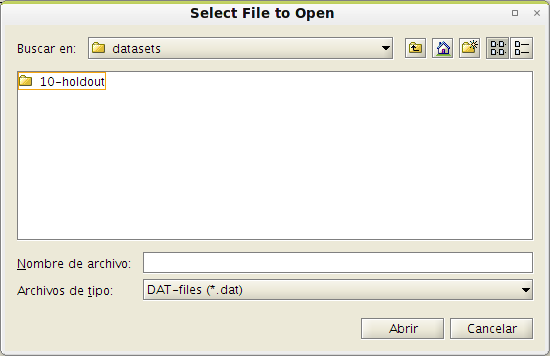
\includegraphics[scale=0.6]{interfaz/interface04.png}
			\caption{Interfaz gráfica. Selección de la carpeta datasets.}
			\label{fig:int04}
		\end{figure}
		
		\begin{figure}[htbp]
			\centering
			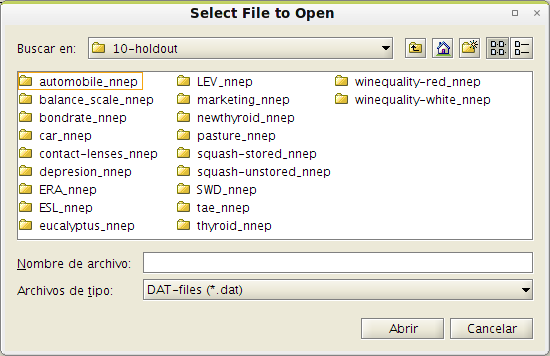
\includegraphics[scale=0.6]{interfaz/interface05.png}
			\caption{Interfaz gráfica. Selección de la carpeta 10-holdout.}
			\label{fig:int05}
		\end{figure}
		
		\begin{figure}[htbp]
			\centering
			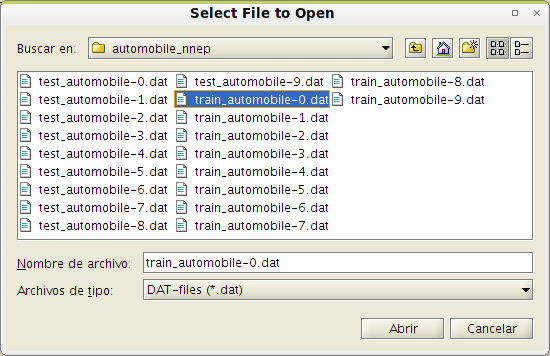
\includegraphics[scale=0.6]{interfaz/interface06.png}
			\caption{Interfaz gráfica. Selección del fichero de entrenamiento.}
			\label{fig:int06}
		\end{figure}
		
		\begin{figure}[htbp]
			\centering
			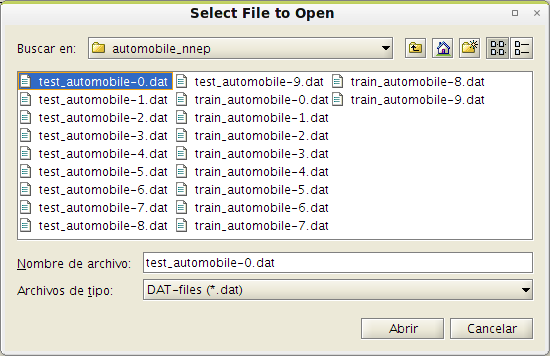
\includegraphics[scale=0.6]{interfaz/interface07.png}
			\caption{Interfaz gráfica. Selección del fichero de test.}
			\label{fig:int07}
		\end{figure}
		
		Una vez seleccionados los datos se mostrará una breve información sobre las dimensiones de los conjuntos de datos en el panel de información de la derecha. La Figura \ref{fig:int08} muestra dicha pantalla con la información del ejemplo cargado. \\
		
		\begin{figure}[htbp]
			\centering
			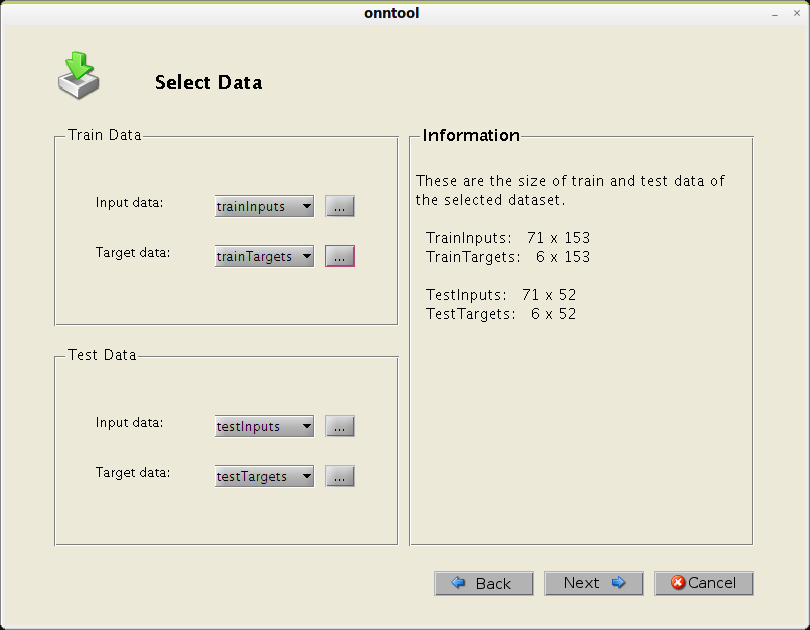
\includegraphics[scale=0.5]{interfaz/interface08.png}
			\caption{Interfaz gráfica. Datos cargados.}
			\label{fig:int08}
		\end{figure}
		
		Si al intentar cargar los datos se produce una equivocación en el fichero de datos o se intenta cargar un fichero con una extensión incorrecta, se mostrará un aviso para que se carguen de nuevo los datos correctos y no se hará nada. Si todo el proceso se ha seguido correctamente se podrá pulsar el botón de siguiente (Next) o de atrás (Back) para navegar entre pantallas.\\
		
		Una vez pulsado el botón para pasar a la siguiente pantalla (Next), se pasará a la pantalla de configuración de la red neuronal ordinal. Esta pantalla está constituida por dos paneles, uno para la configuración de la red propiamente en la parte izquierda y otro que muestra la información de las acciones disponibles en la parte derecha. La Figura \ref{fig:int09} muestra dicha pantalla.\\
		
		\begin{figure}[htbp]
			\centering
			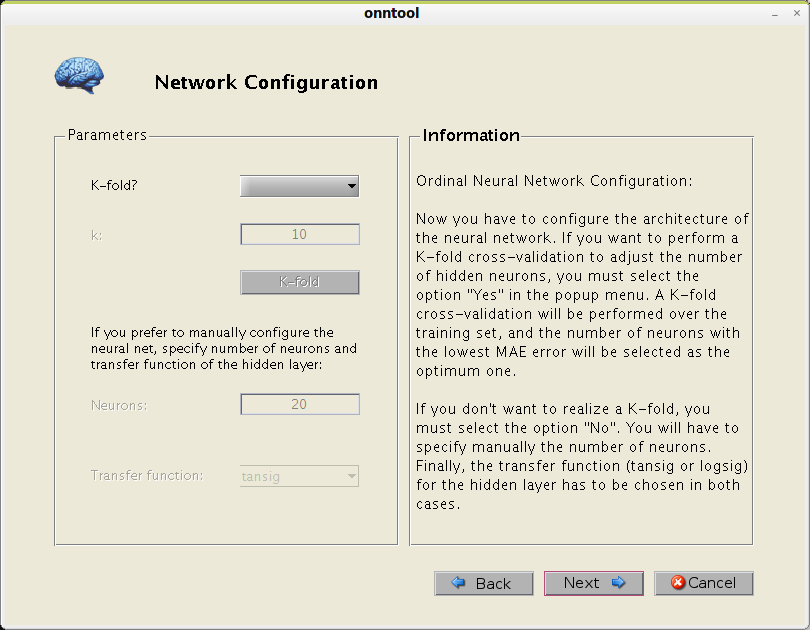
\includegraphics[scale=0.5]{interfaz/interface09.png}
			\caption{Interfaz gráfica. Pantalla de configuración de la red neuronal.}
			\label{fig:int09}
		\end{figure}
		
		En esta pantalla existen dos posibilidades para la configuración de la red neuronal ordinal, la posibilidad de realizar un K-fold cross-validation de los conjuntos de entrenamiento y test para obtener el valor del número de neuronas óptimo de la capa oculta o especificarlo manualmente (20 por defecto). También se tendrá que especificar en ambos casos la función de transferencia a usar, que podrá ser \textit{logsig} o \textit{tansig}. Las Figuras \ref{fig:int10} y \ref{fig:int11} muestran dichas pantallas.\\
		
		\begin{figure}[htbp]
			\centering
			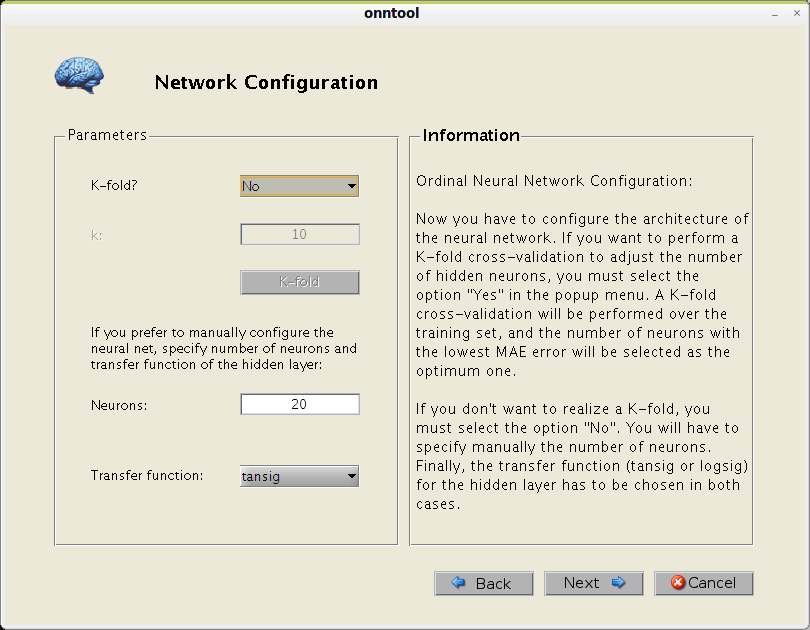
\includegraphics[scale=0.5]{interfaz/interface10.png}
			\caption{Interfaz gráfica. Opción manual de configuración de la red neuronal.}
			\label{fig:int10}
		\end{figure}
		
		\begin{figure}[htbp]
			\centering
			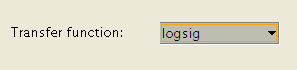
\includegraphics[scale=1]{interfaz/interface11.png}
			\caption{Interfaz gráfica. Opción de función de transferencia.}
			\label{fig:int11}
		\end{figure}
		
		Si se elige la opción de realizar un K-fold, se podrá especificar el valor de \textit{k} (10 por defecto). Una vez seleccionado el valor de \textit{k} habrá que pulsar el botón de K-fold para realizar el proceso. Si se intenta pasar directamente a la siguiente pantalla sin pulsar dicho botón, se mostrará un aviso para que se pulse el botón y se pueda realizar el K-fold. La Figura \ref{fig:int12} muestra dicha pantalla y la Figura \ref{fig:int12-1} muestra el aviso.\\
		
		\begin{figure}[htbp]
			\centering
			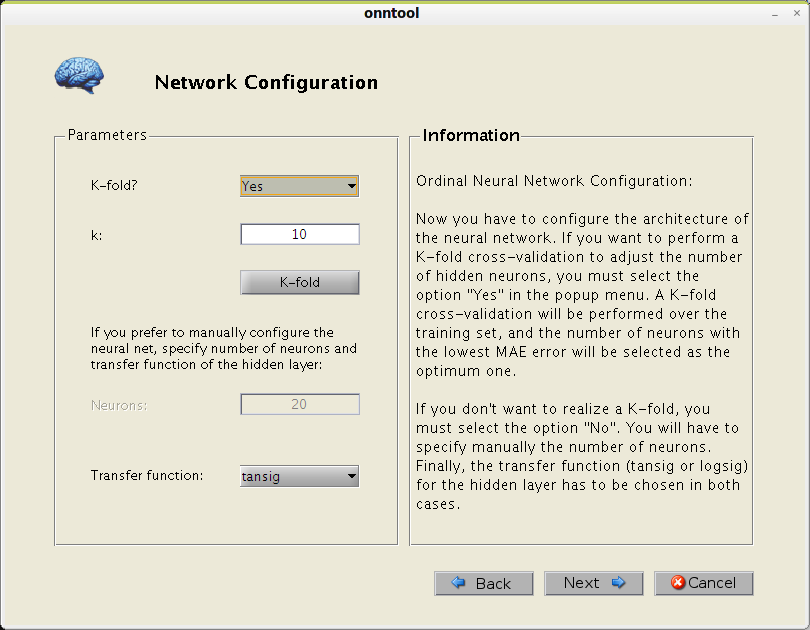
\includegraphics[scale=0.5]{interfaz/interface12.png}
			\caption{Interfaz gráfica. Opción para realizar un K-fold.}
			\label{fig:int12}
		\end{figure}
		
		\begin{figure}[htbp]
			\centering
			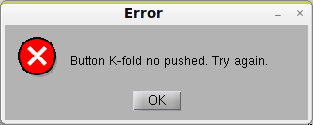
\includegraphics[scale=1]{interfaz/interface12-1.png}
			\caption{Interfaz gráfica. Aviso de la opción K-fold.}
			\label{fig:int12-1}
		\end{figure}
		
		Mientras se realiza el K-fold cross-validation se presentará un mensaje de espera para informar que el proceso está activo. Una vez terminado el proceso, se cerrará el mensaje y se podrá pasar a la siguiente pantalla.\\
		
		\begin{figure}[htbp]
			\centering
			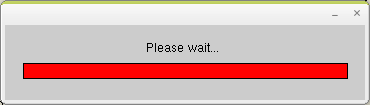
\includegraphics[scale=1]{interfaz/interface12-2.png}
			\caption{Interfaz gráfica. Barra de espera de la opción K-fold.}
			\label{fig:int12-2}
		\end{figure}
		
		Al pasar a la siguiente pantalla, que es la pantalla de entrenamiento, se mostrarán dos nuevos paneles. El primer panel mostrará el botón para realizar el entrenamiento de la red (Train). La Figura \ref{fig:int13} muestra dicha pantalla.\\
		
		\begin{figure}[htbp]
			\centering
			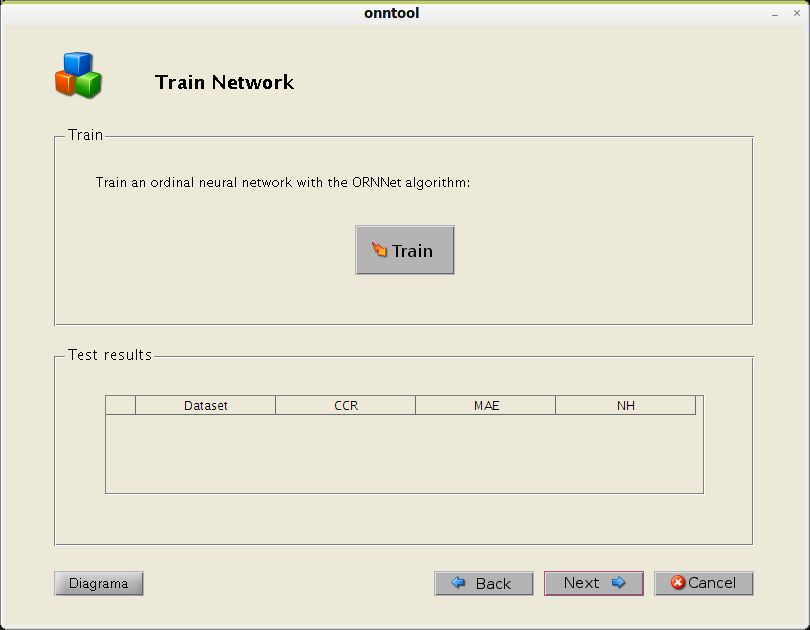
\includegraphics[scale=0.5]{interfaz/interface13.png}
			\caption{Interfaz gráfica. Pantalla de entrenamiento.}
			\label{fig:int13}
		\end{figure}
		
		El segundo panel, en cambio, mostrará los resultados del proceso de entrenamiento y simulación. Adicionalmente, en esta pantalla se añade un nuevo botón para poder ver de manera gráfica la forma de la red neuronal ordinal (Diagram) configurada. El resultado de este ejemplo se muestra en la Figura \ref{fig:int13-1}.\\
		
		\begin{figure}[htbp]
			\centering
			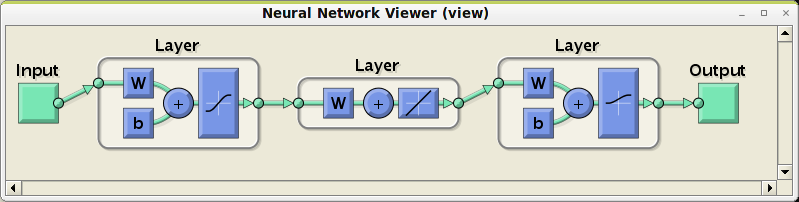
\includegraphics[scale=0.5]{interfaz/interface13-1.png}
			\caption{Interfaz gráfica. Pantalla con red neuronal de forma gráfica.}
			\label{fig:int13-1}
		\end{figure}
		
		Si se pulsa el botón de entrenamiento (Train), se realizará el entrenamiento y la simulación de la red neuronal ordinal con los datos seleccionados y la configuración definida. Además, se mostrarán varias pantallas adicionales que se muestran en las Figuras \ref{fig:int13-2} y \ref{fig:int13-3}. Éstas muestran la matriz de confusión proporcionada para las salidas obtenidas y la pantalla que proporciona el toolbox \textit{nnet} cuando se entrena una red neuronal la cual muestra de forma gráfica, pero en pequeña escala, la red neuronal ordinal, la evolución de algunos parámetros para el entrenamiento y la posibilidad de generar alguna gráfica que mostrará estadísticas de los resultados de entrenamiento.\\
		
		\begin{figure}[htbp]
			\centering
			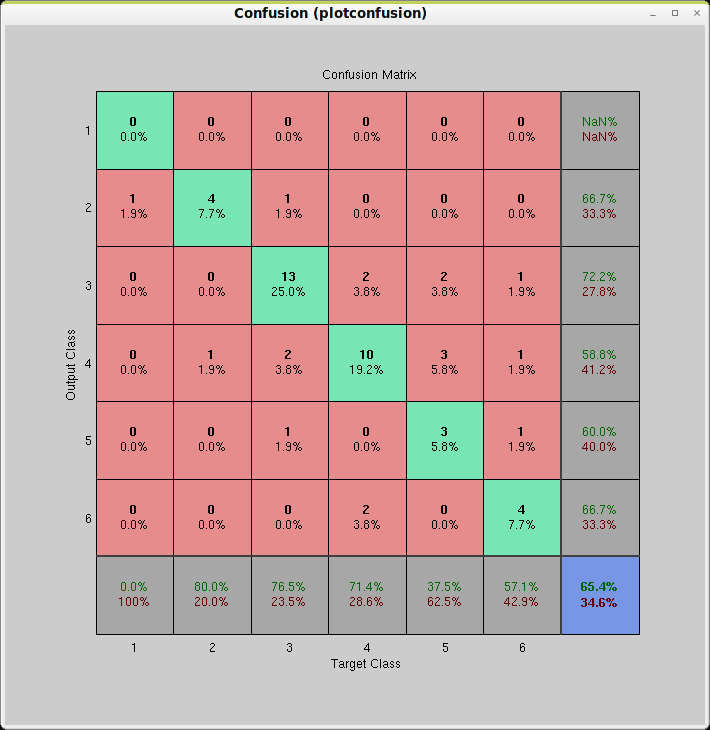
\includegraphics[scale=0.6]{interfaz/interface13-2.png}
			\caption{Interfaz gráfica. Matriz de confusión.}
			\label{fig:int13-2}
		\end{figure}
		
		\begin{figure}[htbp]
			\centering
			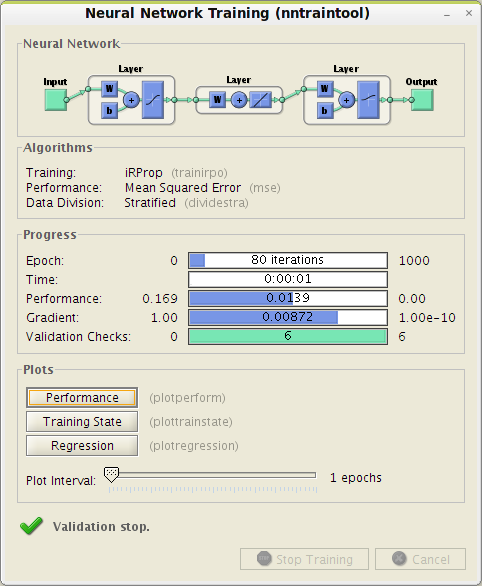
\includegraphics[scale=0.8]{interfaz/interface13-3.png}
			\caption{Interfaz gráfica. Pantalla de entrenamiento de nnet.}
			\label{fig:int13-3}
		\end{figure}
		
		Una vez entrenada la red neuronal ordinal, se rellenará la tabla de resultados como se muestra en la Figura \ref{fig:int14}, en la que se podrá observar los siguientes datos: el nombre del conjunto de datos evaluado, el valor del CCR obtenido, el valor del MAE y el número de neuronas en capa oculta, que será el especificado, en el caso de que la configuración haya sido manual, o un valor $2^n$ con $n = 0,...,5$. Adicionalmente, se podrá observar que el botón de entrenamiento habrá cambiado (Retrain) para poder reentrenar la red neuronal.\\
		
		\begin{figure}[htbp]
			\centering
			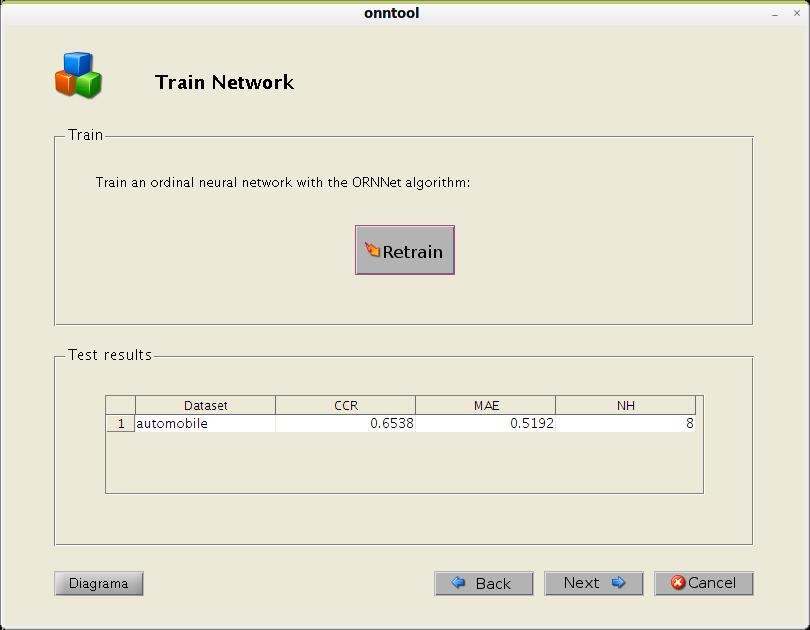
\includegraphics[scale=0.5]{interfaz/interface14.png}
			\caption{Interfaz gráfica. Muestra de los resultados obtenidos.}
			\label{fig:int14}
		\end{figure}
		
		Por último, al pulsar de nuevo el botón de siguiente (Next) se pasará a la siguiente pantalla, la pantalla de exportado de datos en el \textit{workspace} de Matlab. La Figura \ref{fig:int15} muestra dicha pantalla, la cual contiene un panel en el que se podrá especificar el nombre de las variables a exportar. Los datos que se podrán exportar son: la red neuronal ordinal, las salidas obtenidas al aplicar el algoritmo ORNNet y los resultados (CCR, MAE y NH). Tendrá la opción de exportar las variables o no según desee, en caso afirmativo habrá que pulsar el botón correspondiente. Por último, existirá un nuevo botón para poder finalizar y cerrar la aplicación (Finish).\\
		
		\begin{figure}[htbp]
			\centering
			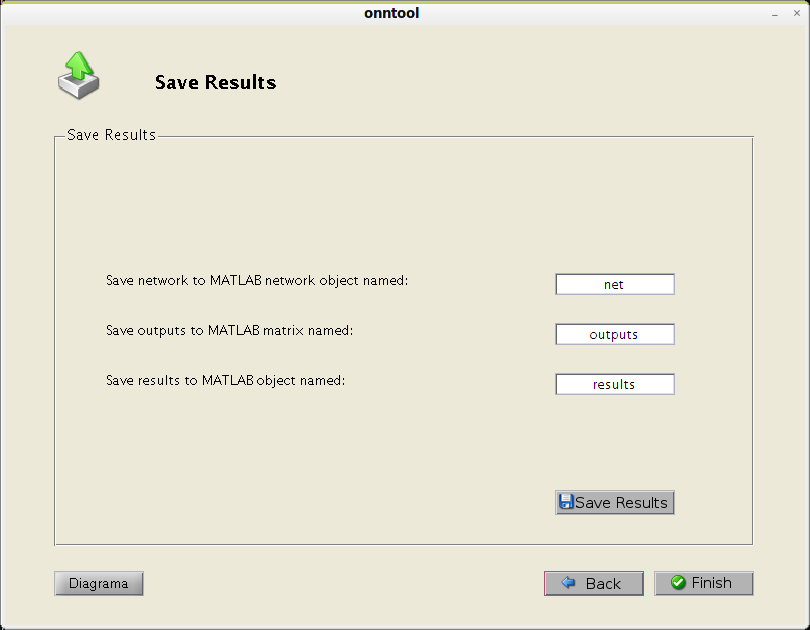
\includegraphics[scale=0.5]{interfaz/interface15.png}
			\caption{Interfaz gráfica. Pantalla de guardado de datos.}
			\label{fig:int15}
		\end{figure}
		
		Comentar que, como se ha observado en las distintas pantallas, se podrá navegar hacia adelante o hacia atrás por las pantallas en todo momento, mientras que todos los parámetros se encuentren especificados o no se pulse el botón de finalización (Finish), lo que facilita la modificación dinámica en todo momento de la aplicación, pudiendo obtener y visualizar nuevos resultados de otros conjuntos de datos u otra configuración de la red neuronal ordinal.
